\documentclass[tikz,border=10pt]{standalone}
\usetikzlibrary{intersections,calc}

\begin{document}
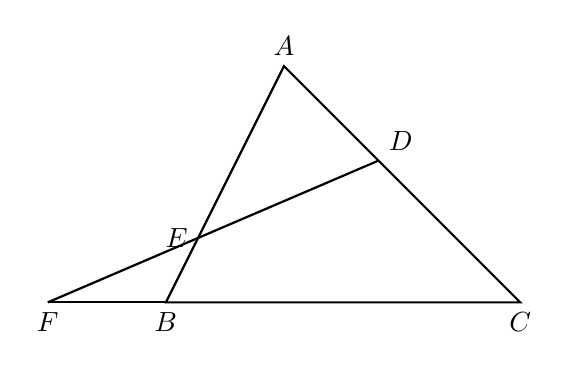
\begin{tikzpicture}[scale=1.5,thick]
    % 1. 定义坐标
    \coordinate (B) at (0,0);
    \coordinate (C) at (3,0);
    \coordinate (A) at (1,2);
    % 定义 F 在 CB 延长线上
    \coordinate (F) at (-1,0); 
    
    % 2. 定义线段 D 在 AC 上
    \coordinate (D) at ($(A)!0.4!(C)$); % D 位于 AC 的 0.4 处
    
    % 3. 绘制三角形及主要线段
    \draw (A) -- (B) -- (C) -- cycle; % 三角形 ABC
    \draw (F) -- (D);                % 线段 FD
 \draw (F) -- (B);       
    
    % 4. 计算交点 E
    \coordinate (E) at (intersection of A--B and F--D);
    
    % 5. 标注点位
    \node[above] at (A) {$A$};
    \node[below] at (B) {$B$};
    \node[below] at (C) {$C$};
    \node[below] at (F) {$F$};
    \node[above right] at (D) {$D$};
    \node[left] at (E) {$E$};
    
\end{tikzpicture}
\end{document}